%%%%%%%%%%%%%%%%%%%%%%%%%%%%%%%%%%%%%%%%%%%%%%%%%%%%%%%%%%%%%%%%%%%%%%%%%%%%%
% Rich Meier 3/15/14 - Final Project - UCT Monte Carlo Othello Project %%%%%%%%%%%%%%%%%%%%%%%%%%%%%%%%%%%%%%%%%%%%%%%%%%%%%%%%%%%%%%%%%%%%%%%%%%%%%%
% Header
\documentclass[12pt,letterpaper]{article}
\usepackage[utf8]{inputenc}
\usepackage{amsmath}
\usepackage{amsfonts}
\usepackage{amssymb}
\usepackage{graphicx}
\usepackage[margin=1in]{geometry}
%\usepackage{booktabs}
%\usepackage{colortbl}
%%%%%%%%%%%%%%%%%%%%%%%%%%%%%%%%%%%%%%%%%%%%%%%%%%%%%%%%%%%%%%%%%%%%%%%%%%%%%%
%\definecolor{grey}{RGB}{190,190,190}
% Begin
\begin{document}

\title{\vspace{-1in}Final Project -- CS 533 \\ Monte Carlo UCT Algorithm Applied to Playing Othello}
\author{Rich Meier \& Austin Sharp}
\date{\today}
\maketitle

\vspace{-.5in}
\section{Introduction}
The following report will cover the development of a Monte-Carlo-based Othello player. The algorithm described below will use the UCT algorithm to play Othello against multiple opponents in a adversarial environment. We have developed the UCT Monte-Carlo-based tree search algorithm in python, and created it to be compatible with a pre-designed Othello game environment. The hope is that our algorithm will succeed in beating the provided AI that uses a minimax search of variable depth with alpha-beta pruning.

Section~\ref{back} will provide some fundamental background knowledge on the game Othello, as well as the theoretical components of the UCT tree algorithm.  Next, Section~\ref{meth} will cover the methodology and important coding used to validate and evaluate our algorithm. Section~\ref{results} will discuss the results of the experimentation described in the previous section, and finally Section~\ref{conc} will conclude.

\section{Background Information}
\label{back}

The following discusses the fundamental components of playing Othello, as well as implementing the UCT algorithm.

\subsection{Playing Othello}

The game of Othello is actually quite simple. It is a two player game where each player seeks to maximize the number of chips on the board that are their own color (black or white). The board is typically an eight by eight square, and play continues on the board while either player still has a legal move or until the board is full. Legal moves must have at least one adjacent token that is the opponent's color, and the current player's own color is either diagonally, vertically, or horizontally aligned with the move.  

In order to maximize the number of captured pieces on the board, there are a few widely accepted strategic positions.  Specifically, capturing corner squares is considered best because they are impossible for the opposing player to recapture. Side squares are also advantageous because the eliminate capturing capability in the orthogonal direction. Figure~\ref{fig1} depicts a typical Othello game in progress.

Overall, Othello is considered a difficult game for humans, because results may swing wildly at the end of the game based on large captures made by a few placements of pieces, and it is hard to predict these outcomes from early game positions. As a result, it is ideal for automated planning. Additionally, the large branching factor when there are many possible moves means that estimating Q-values is a valid and logical approach, as is done in UCT.

\begin{figure}[!h]
\begin{center}
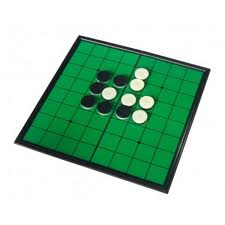
\includegraphics[scale=1]{othello_board}
\caption{\textit{The Othello game -- a mid-game snapshot.}}
\label{fig1}
\end{center}
\end{figure}

\pagebreak
\subsection{UCT Algorithm}
The UCT algorithm is a Monte-Carlo tree based algorithm that utilizes explore/exploit tactics to build a decision tree at each independent action level. Simply put, whenever the agent must make a decision, the UCT algorithm rolls-out multitudes of independent trajectories that utilize the best policy according to the tree. If the trajectory reaches a point that the tree has not yet simulated, a default policy is executed in order to simply estimate values for that particular sub-tree.  This in turn adds and updates a new leaf node as well as the nodes along the path of the trajectory from the leaf node up to the root.

The values that are learned via this algorithm are approximate Q-values.  This means that node has a value that is specifically related to both the state of the game at that point, as well as ``best" action that the agent can take at that point. When moving through already-explored nodes, the UCT algorithm's tree policy will choose the next action based on a summation of the best known Q-value and an exploring value (based on how many times each action is taken).  This is represented by the policy relationship in Equation~\ref{eq1} below:
\begin{equation}
\label{eq1}
\Pi_{uct}(s) = MAX_a \left( Q(s,a) + c*\sqrt{\frac{\log(n(s))}{n(s,a)}} \right)
\end{equation}

Ultimately the actual decision chosen by UCT is the action with the highest Q-value at the root node - disregarding the exploration term. A new tree is built at each step where the agent must make a decision.

\pagebreak
\section{Methodology}
\label{meth}

\subsection{Othello Python Code}

A 3rd-party Othello environment was used for simulation and competition. Some small changes were made to the code in order to implement UCT and use it as an agent in the Othello environment.

The 3rd-party environment is centered around `othello.py', which contains the class `game'. This class maintains the Othello board, describes whose turn it is, enumerates the moves that are available, and allows moves to be played. It also keeps score (that being the difference between the number of pieces of black and white on the board). The file `game2.py' provides the `player' class, which is initialized with a policy function (that takes a position and returns a move). Game2.py also provides a play() function which takes a game state and two players and simulates the rest of the game. We modified play() to return the final score of the game, since it is helpful to know who wins after simulating a game. 

This the entire simulator environment. However, there are two more files that were included with this package: `othello\_gui.py', which provides a simple GUI for a human to play against any opponent player, and `minimax.py', which implements an agent that uses minimax alpha-beta search with a variable lookahead depth and a custom evaluation function. This minimax agent, was implemented using a more traditional AI method, and it was a useful benchmark for us in evaluating the performance of our agent.

\subsection{Custom Code}

Our code consists of two files. CS533\_Final.py is the file that runs simulations and was used for experiments. It also contains some simple policies, one random policy that chooses from the available moves, and one greedy policy that chooses the move that will capture the greatest number of the opponent's pieces. These simple policies were the two available default policies for our simulations (playing against themselves) in UCT.

UCT\_tree.py is the file that contains the bulk of the UCT algorithm. Overall it is almost independent of the game of Othello, relying only on generic functions of the simulator such as the game class' generate\_moves() and play\_move() functions, as well as access to a simulator that returns the overall reward. The class Tree consists of a list of nodes, as well as some parameters of the UCT algorithm: the time budget per move, the value c of the tree policy, and the policy function to be used when simulating results.

Each node corresponds to a certain state (and contains a game object). Nodes keep track of their children (by indices of the children in the tree's list of nodes), the number of times each action was taken, and the rewards received from simulations following those actions. Nodes can also calculate the value of their actions according to the UCT tree policy (when given a value for c) as well as the estimated reward from each action.

The tree class builds a tree of nodes over many simulated trajectories and relies upon them to decide the best action. This begins in the policy() function, which runs trajectories from the root node until the time allotted runs out, and then picks the move with the highest Q-value.

The trajectory() function is the most involved, and does most of the tree building. At a given node, trajectory() will first check if all of the nodes' actions have been taken at least once. If some have not, it randomly chooses one, takes that action, adds a new node to the tree, and simulates the game from that new node based on the default policy (random or greedy). If all actions have been taken, trajectory() uses the tree policy and its explore-exploit nature to choose an action to take, and recursively calls trajectory on the node resulting from that action, which will eventually lead to the base case, where trajectory is called on a node with some actions that have not yet been simulated. In the base case, the resulting reward from the simulation is returned and used to update the action counts and action rewards on each node, and this is propagated up the tree as the recursion unwinds.

Our implementation incidentally relies on the fact that Othello is deterministic, so once an action leads to a child node (that is, a game state), it will always lead there. For a nondeterministic simulation, this would need to be replaced by a mapping between game states and node indices. Otherwise our entire implementation could be reused on a simulator of an entirely unrelated game.

Finally, our evaluation in CS533\_Final.py consists of nested loops over several sets of parameters, including the default policy, opponent players, values of c, time budgets per-move, and the number of games to play at each configuration. This makes it easy to collect results for any number of possible configurations. However, especially with larger time budgets, the runtime becomes prohibitive, and thus we used this setup to select interesting values, to cut down on the number of final configurations tested.

\subsection{Experimentation}
As described above, 'CS533\_Final.py' contains the main function that sets up the experimentation, evaluation, and algorithm analysis portion of this project. Below we provide some detail about our experimental setup in order to better understand the Results section of this report.

\subsubsection{Finding UCT C-value} 
Mainly due to extremely long runtime, we decided to determine a sufficient C-value based on a subset of test runs. Here we decided to base our explore/exploit coefficient off of playing the most intelligent opponent that our algorithm would eventually play - namely Minimax lookahead 4 (Minimax-4). Since we planned to run our algorithm on two different board sizes, it was expected that the value of C would change. Since the C is meant to balance Q-values with exploration, it was important to find two independent C-values for both 6x6 and 8x8 because Q-values in 8x8 have the capability to be larger than 6x6 (64 points versus 36 points).  The table below depicts our experimentation for finding a sufficient C-value.

\begin{tabular}{|c|c|c|c|c|}
\hline
C-Value & \multicolumn{4}{c|}{Margin of Victory}\\
\hline 
 & 6x6 as Black & 6x6 as White & 8x8 as Black & 8x8 as White \\ 
\hline 
1 & 4 & 30 & - & - \\ 
\hline 
5 & 11 & 30 & - & - \\ 
\hline 
10 & 3 & 30 & - & - \\ 
\hline 
20 & 17 & 29 & 37 & 41 \\ 
\hline 
30 & 6 & 27 & - & - \\ 
\hline 
35 & 7 & 31 & - & - \\ 
\hline 
40 & 11 & 30 & 35 & 40 \\ 
\hline 
45 & 15 & 28 & - & - \\ 
\hline 
50 & 17 & 33 & 35 & 40 \\ 
\hline 
60 & 2 & 32 & 36 & 36 \\ 
\hline 
70 & - & - & 34 & 46 \\ 
\hline 
80 & 15 & 30 & 30 & 49 \\ 
\hline 
100 & 11 & 32 & 27 & 51 \\ 
\hline 
\end{tabular} 

Based on these simulation results, we determined that the best C-value for a 6x6 board was between $40$ and $50$.  The 8x8 grid had a higher target C-value as expected, and fell in the range $\approx60$ to $80$.  For the 6x6 grid we chose to use $C=45$ and for the 8x8 we chose $C=70$.

\subsubsection{Time Budget}
Since the UCT algorithm results in estimated Q-values, there is no point at which it can be said to be 'done' or 'solved' or 'finished'. Thus at each move, UCT is given a time budget in seconds of how long it may think and run trajectories to improve its estimates. Once the time is up, it must pick an action from the root node. We tested with time budgets of 0.1, 1, and 10 seconds to show in which situations more time to ``think" and run trajectories was necessary.

\subsubsection{Default Policy Choice}
The default policy is used by UCT to simulate trajectories that are outside the UCT tree. In each case, the default policy was used to initialize both players in an Othello game at the state just outside the tree, and then those policies played until the game ended and a result was returned.

Two default policies were used, and both were fairly simple, implemented with very little knowledge of Othello. The first policy is entirely random, choosing one of the available moves at each timestep with no bias or judgment involved. The second policy was greedy, which for a given position always chose the action that would capture the greatest number of the opponent's pieces.

\subsubsection{Varied Opponents}
To evaluate the performance of our UCT-based Othello agent, we played games against a sample of five opponents. The first two opponents were the naive random and greedy policies detailed above, which were intended to be easy to surmount. The other three policies were versions of the minimax search using alpha-beta pruning that was included with the third-party Othello environment we used. The parameter that differed among these minimax opponents was the search depth: we played against opponents that searched to depth 2, 3 and 4.

\subsubsection{Simulating as Black or White (Player 1 or Player 2)}
In Othello, going first or second makes a major difference. The black player goes first, but it is generally considered an advantage to go second - it has been shown that with perfect play by both sides, the player going second will win on a 4x4 or 6x6 board, while perfect play results in a draw on 8x8. In our experiment we simulated 10 games as the black player and 10 games as white for each combination of opponent, budget, and default policy.

\section{Results}
\label{results}

This section will present the results of our experimentation with the UCT algorithm. Each of the graphs below correspond to running the UCT algorithm against a different opponent.  The first five graphs depict the results of playing the game on a 6x6 board size, and the second set of 5 graphs depict the results on a regular-sized 8x8 board.

The graphs are fairly self-explanatory, but there are a few points that should be reiterated for clarity.  First, each graph has 3 main columns that represent the varying budgets of ``think-time per move" for the UCT algorithm.  As explained in our experimentation, we allowed the UCT algorithm 0.1, 1, and 10 seconds to think. Within each major column there are 4 bars.  In Othello, the black player always moves first and white moves second -- this is represented by the color of each bar, where our UCT algorithm is varied between player 1 (black) and player 2 (white). 

The scoring along the y-axis corresponds to the number of captured pieces on the board. In actuality, our experiments averaged the scores over ten games, so each bar represents the average margin of victory over $10$ full games. On a 6x6 board, the best scenario is that our algorithm wins by capturing all $36$ squares on the board, and the worst case is that we receive a score of $-36$ which means that our opponent captured every square on the board. Though perhaps obvious, it is worth mentioning that Othello scoring is binary. For example, on an 8x8 board, there are 64 possible points, if our algorithm gets a score of 40 then we know we beat the opponent by 40 points and thus scoring would be:
\begin{center}
$$\textnormal{Let } X = \textnormal{ Opponent Score} $$
$$\textnormal{Let } Y = \textnormal{ UCT Score} $$
$$ 64 = X+Y = X+(X+40) = 2*X + 40$$ 
Thus:
$$ X = 12 \textnormal{  And   } Y = X+40 = 52$$ 
\end{center}

\begin{figure}[!hp]
\begin{center}
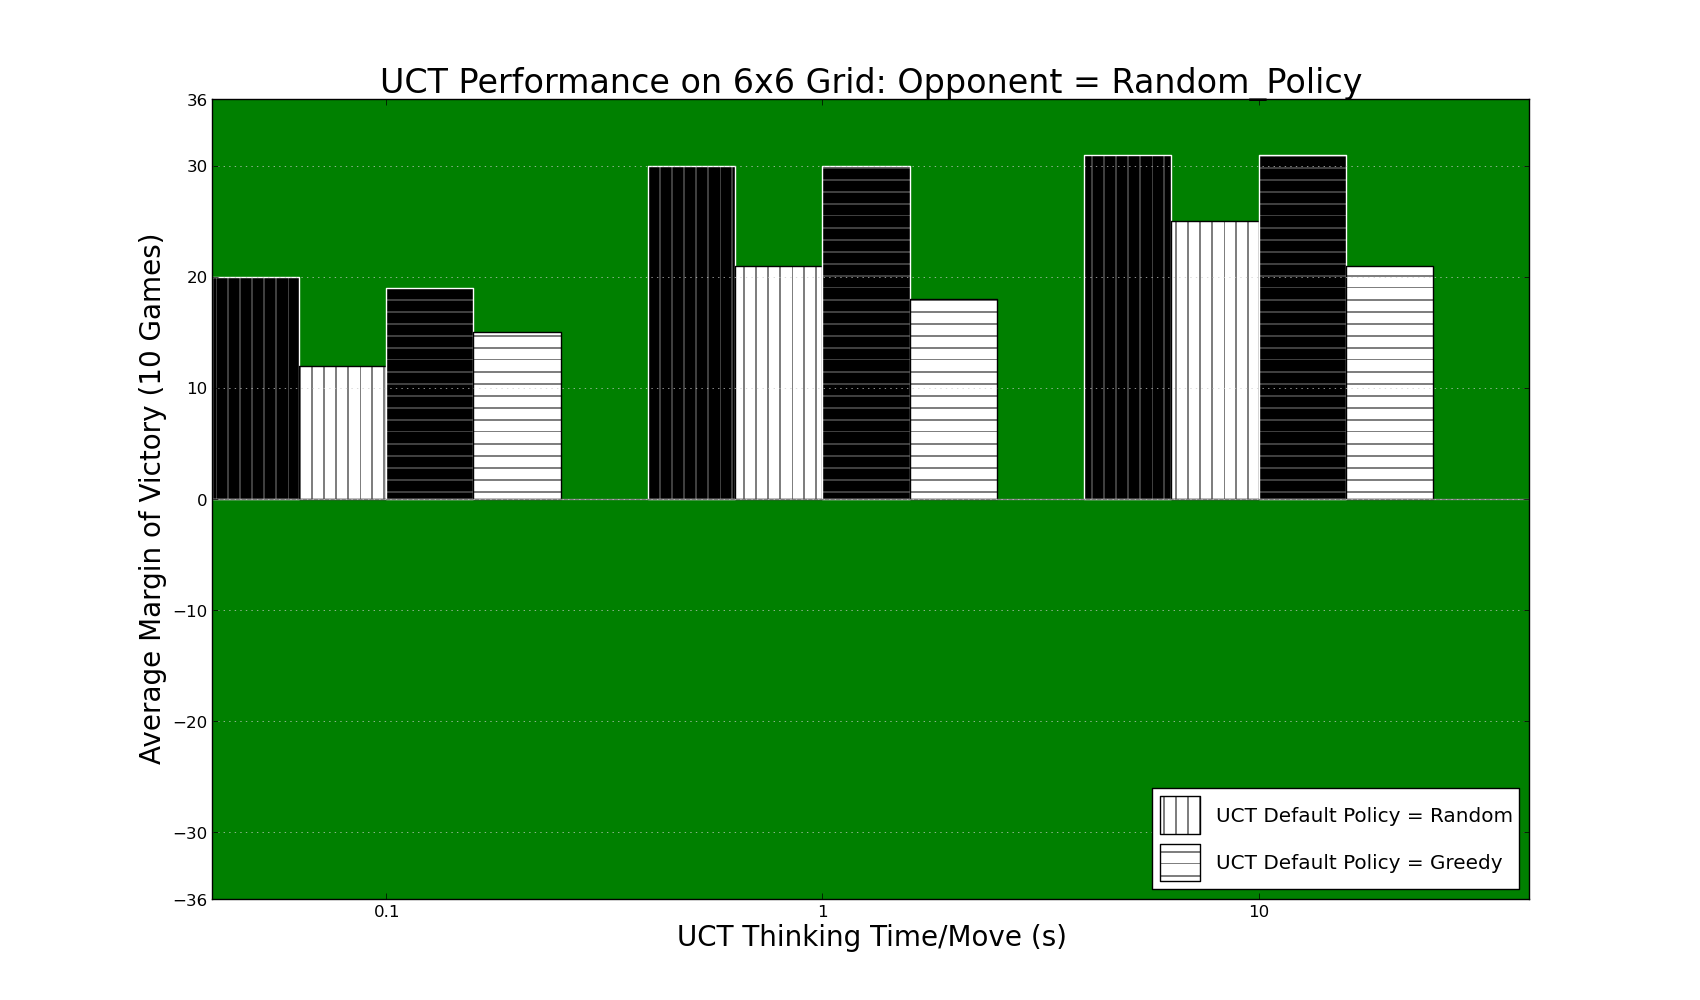
\includegraphics[scale=.4]{66_Random_Policy}
\end{center}
\end{figure}

\begin{figure}[!hp]
\begin{center}
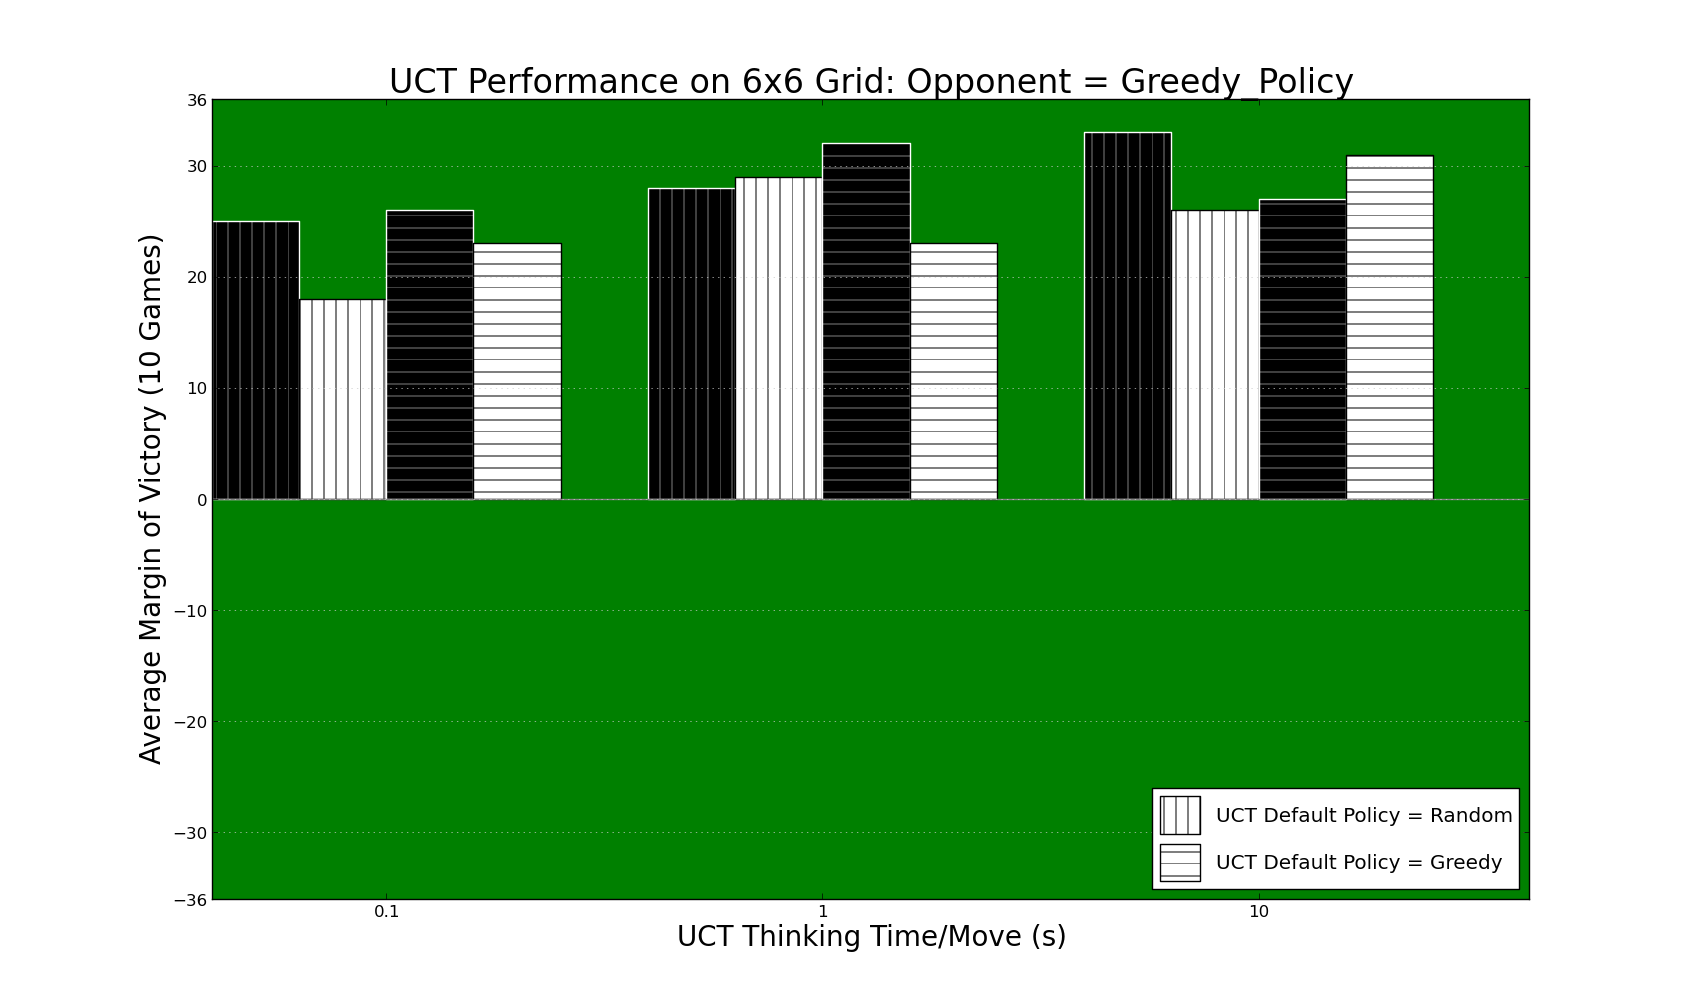
\includegraphics[scale=.4]{66_Greedy_Policy}
\end{center}
\end{figure}

\begin{figure}[!hp]
\begin{center}
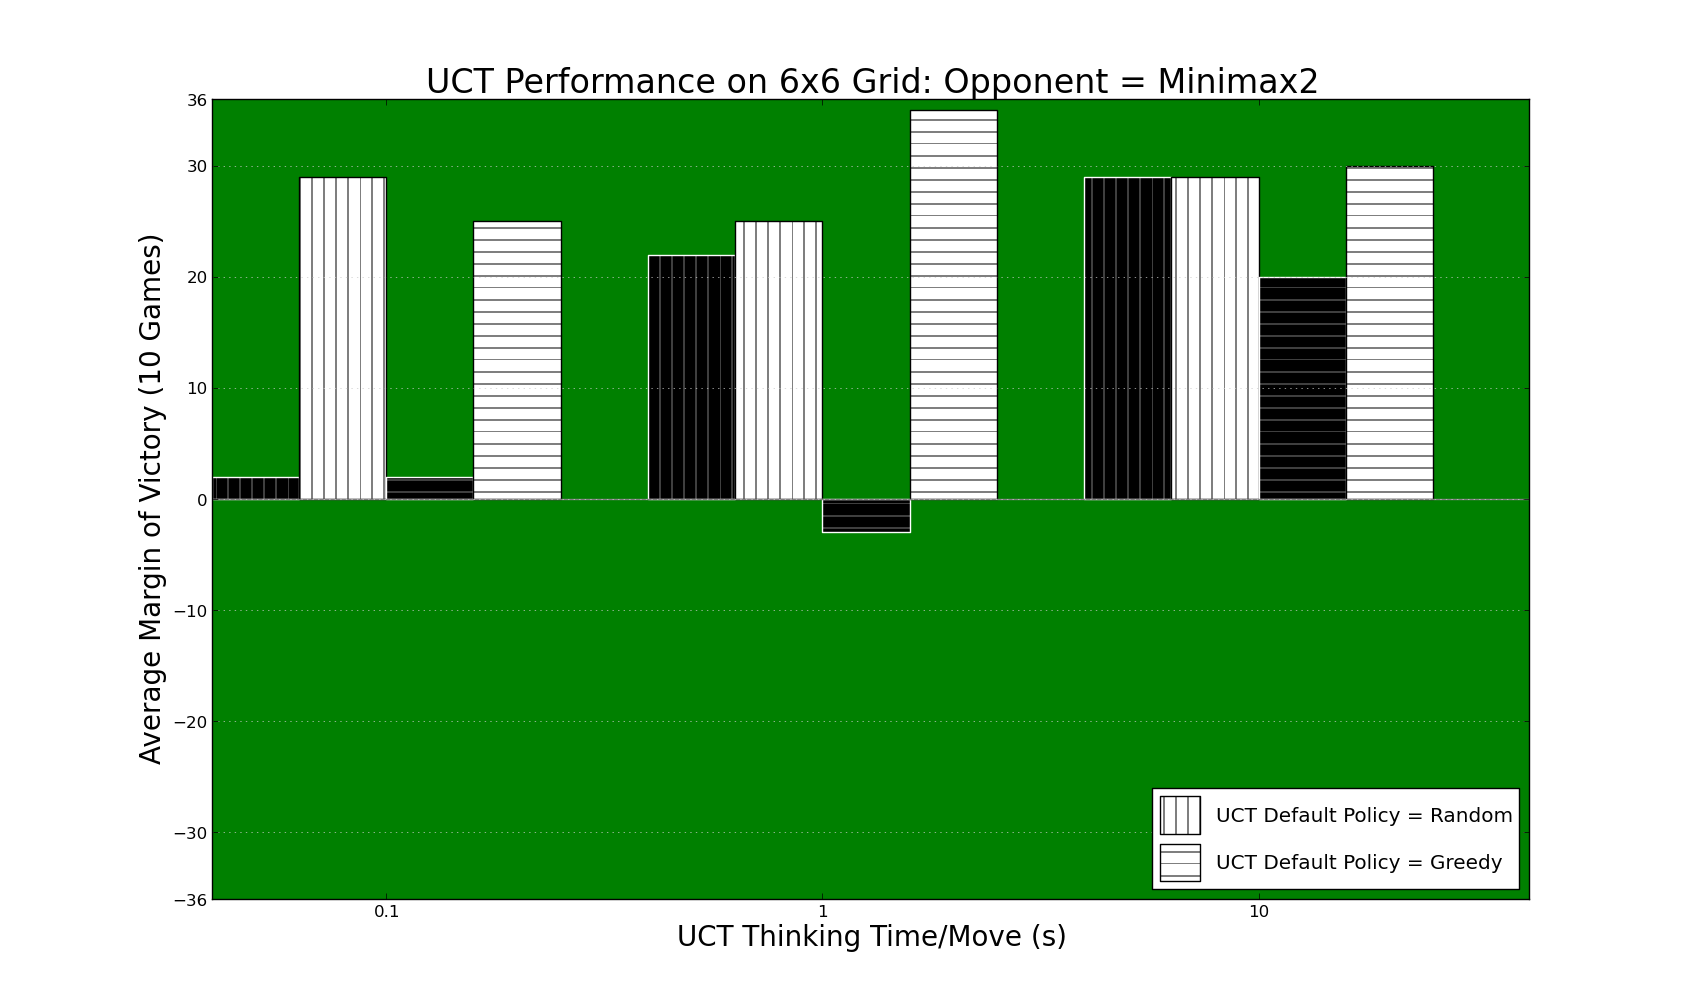
\includegraphics[scale=.4]{66_Minimax2}
\end{center}
\end{figure}

\begin{figure}[!hp]
\begin{center}
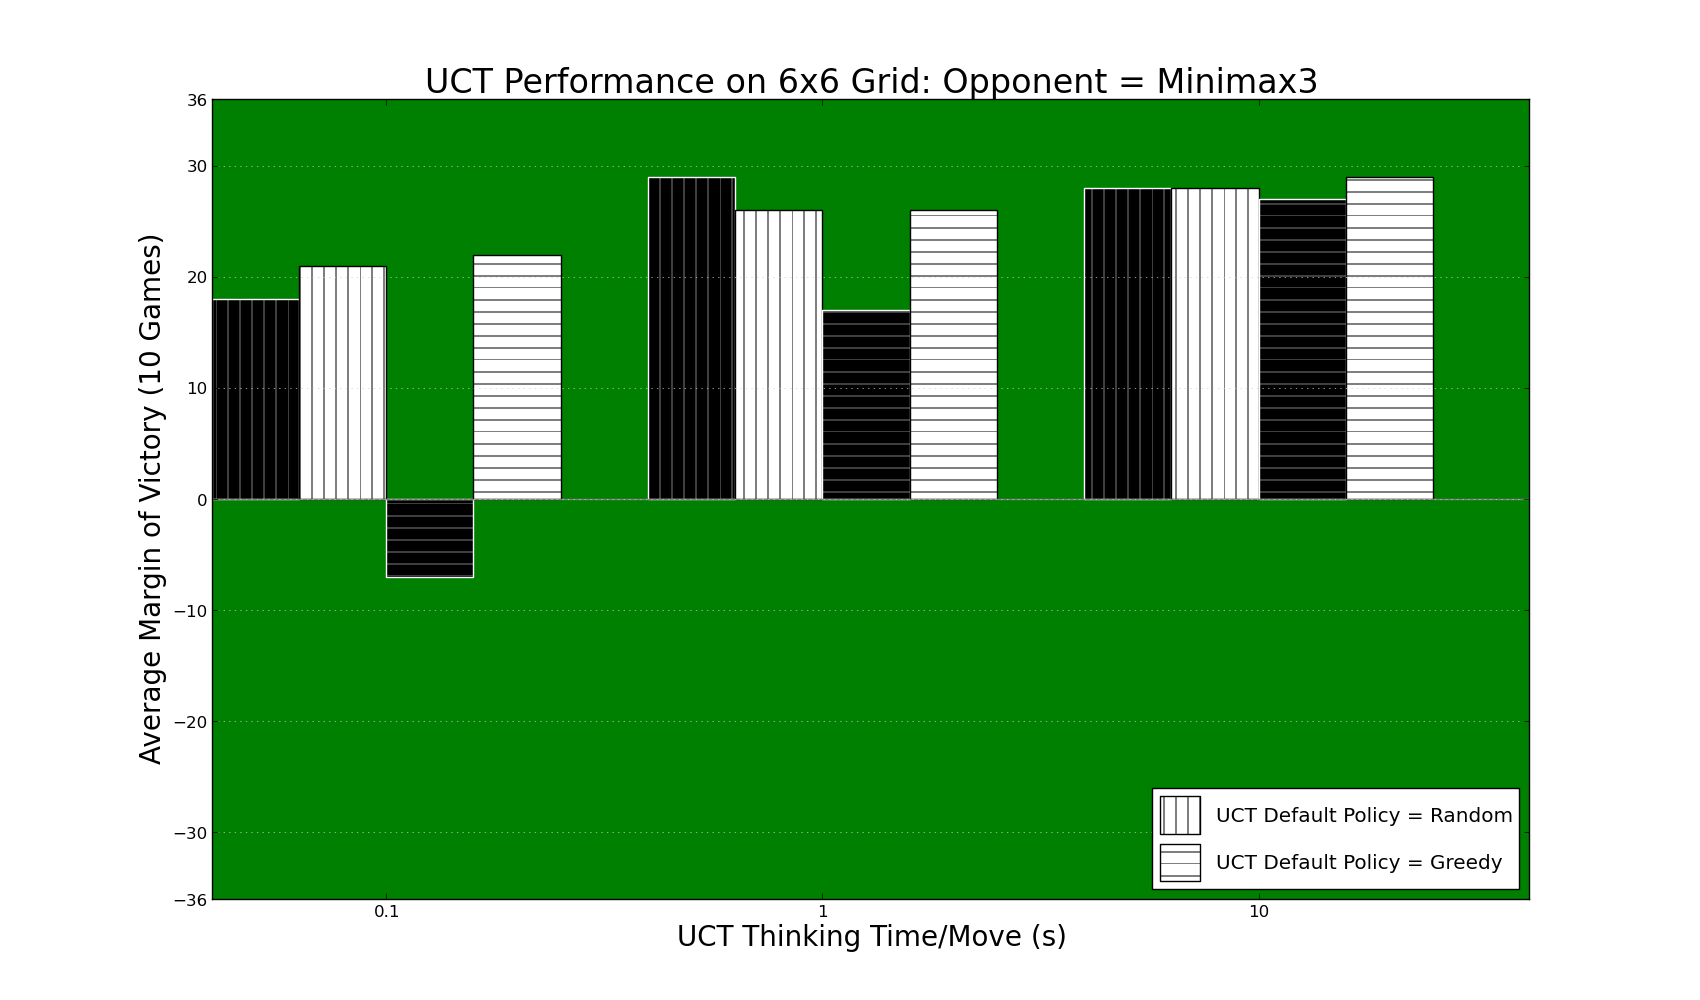
\includegraphics[scale=.4]{66_Minimax3}
\end{center}
\end{figure}

\begin{figure}[!h]
\begin{center}
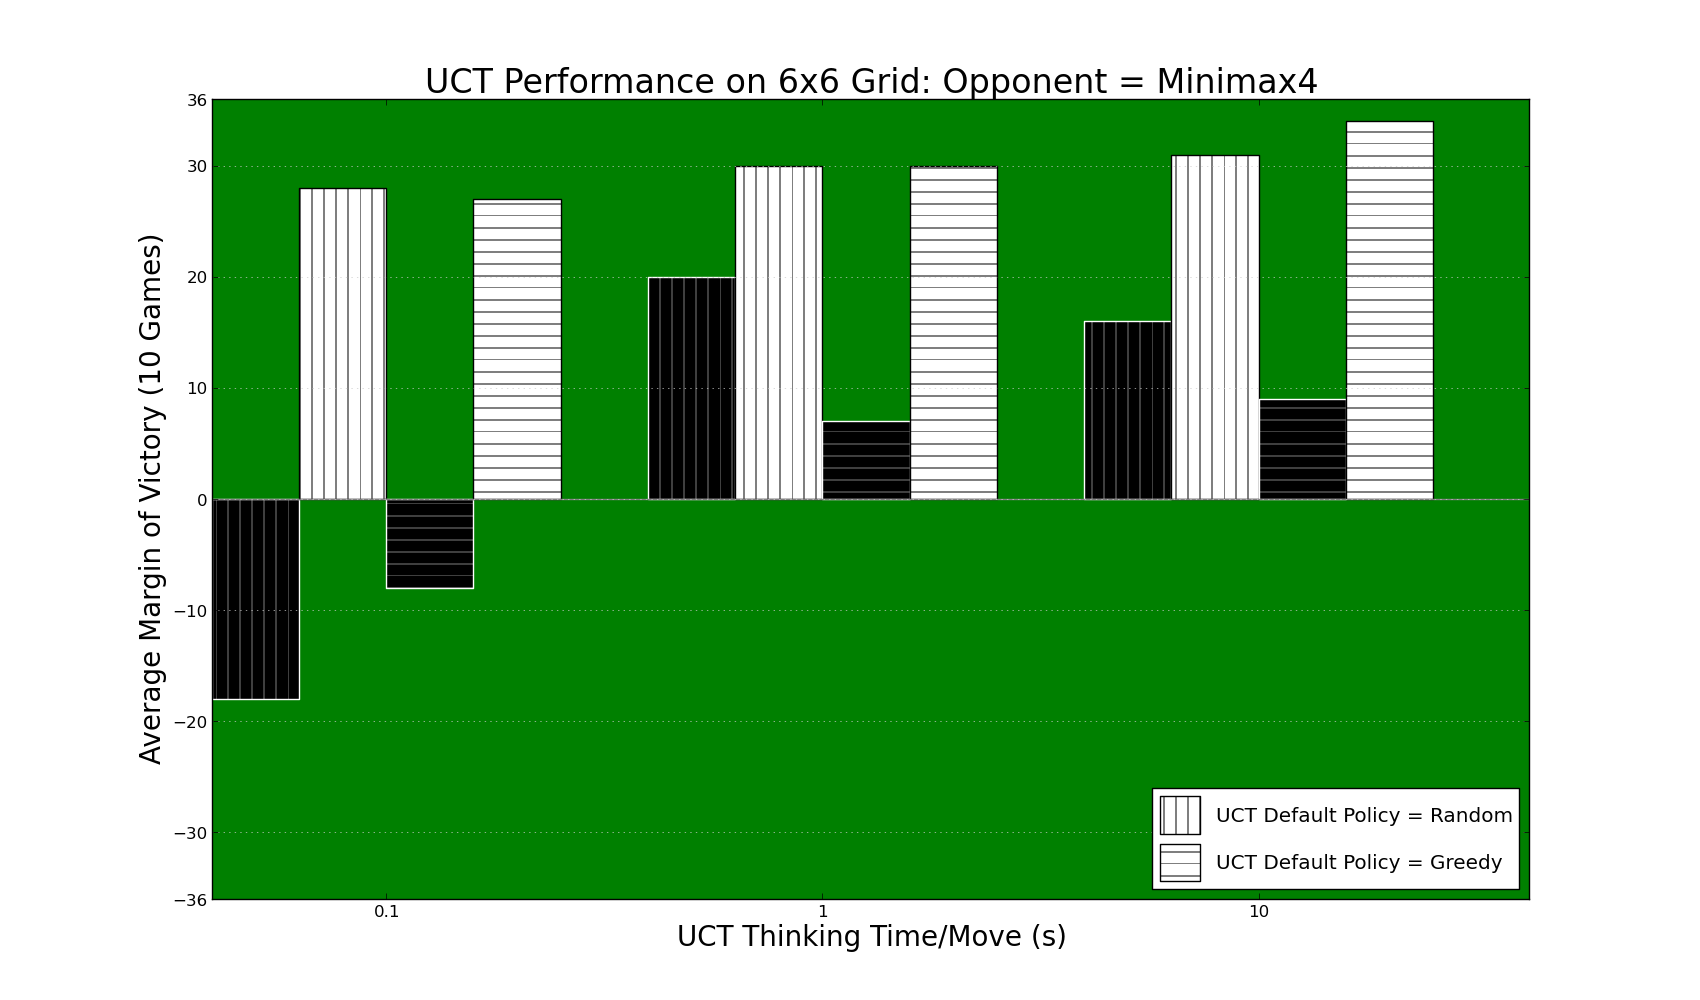
\includegraphics[scale=.4]{66_Minimax4}
\end{center}
\end{figure}

\pagebreak

\begin{figure}[!hp]
\begin{center}
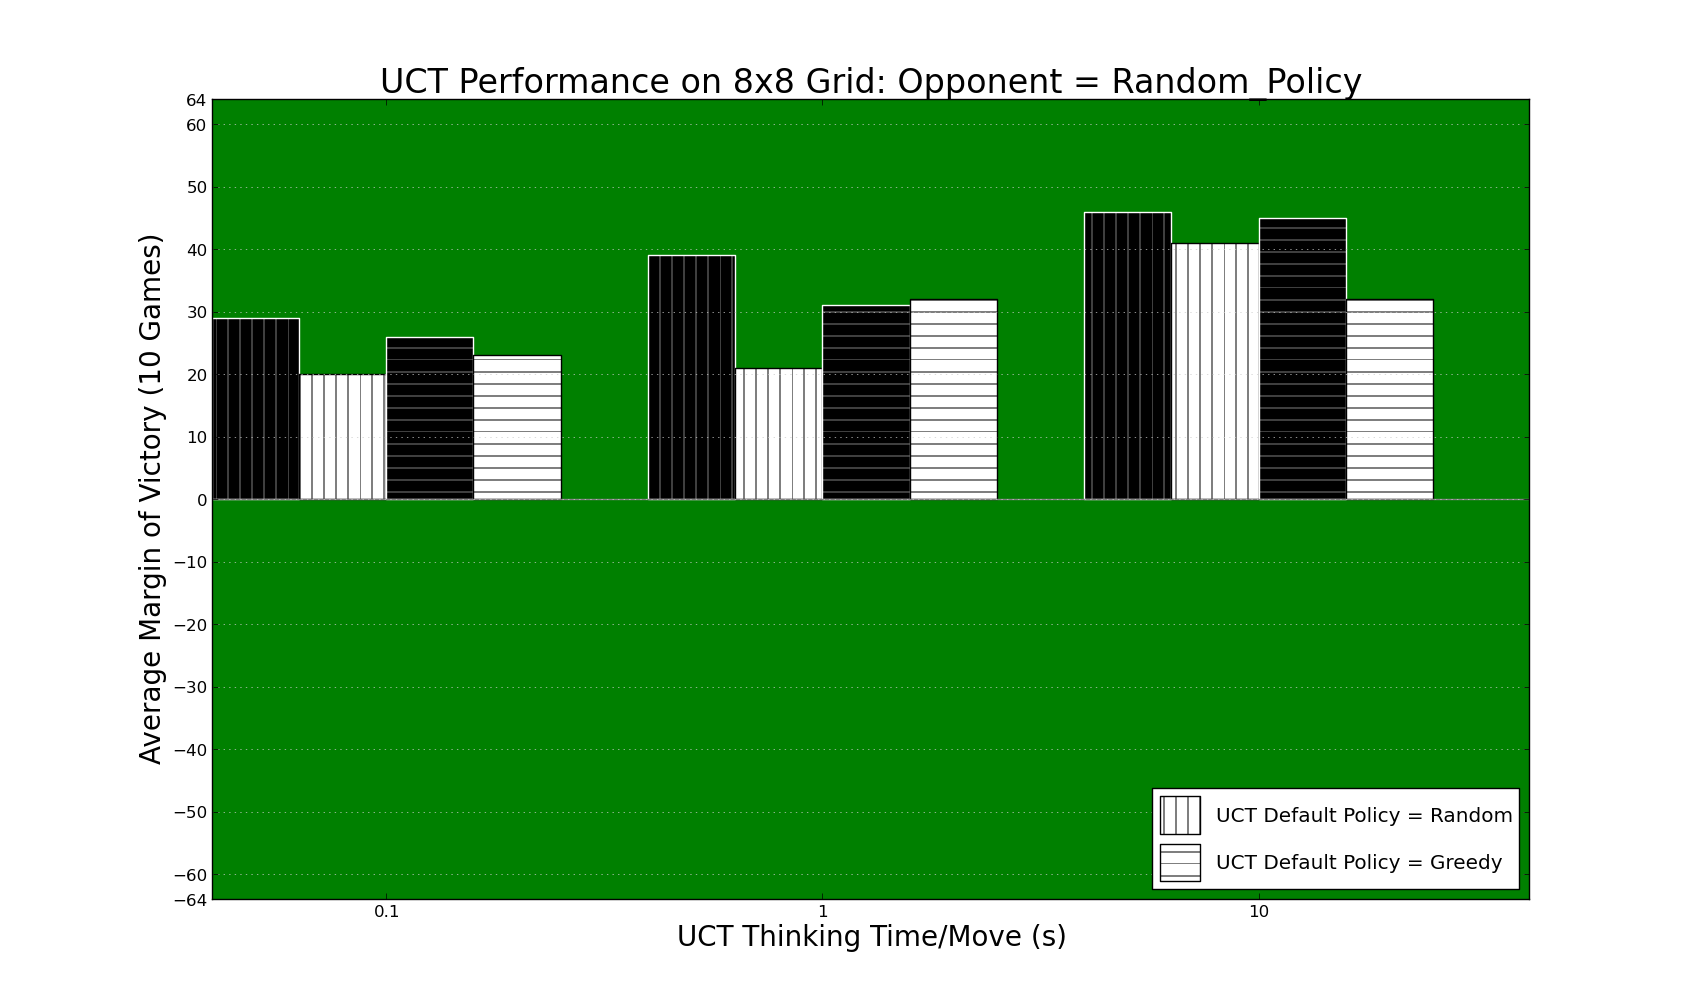
\includegraphics[scale=.4]{88_Random_Policy}
\end{center}
\end{figure}

\begin{figure}[!hp]
\begin{center}
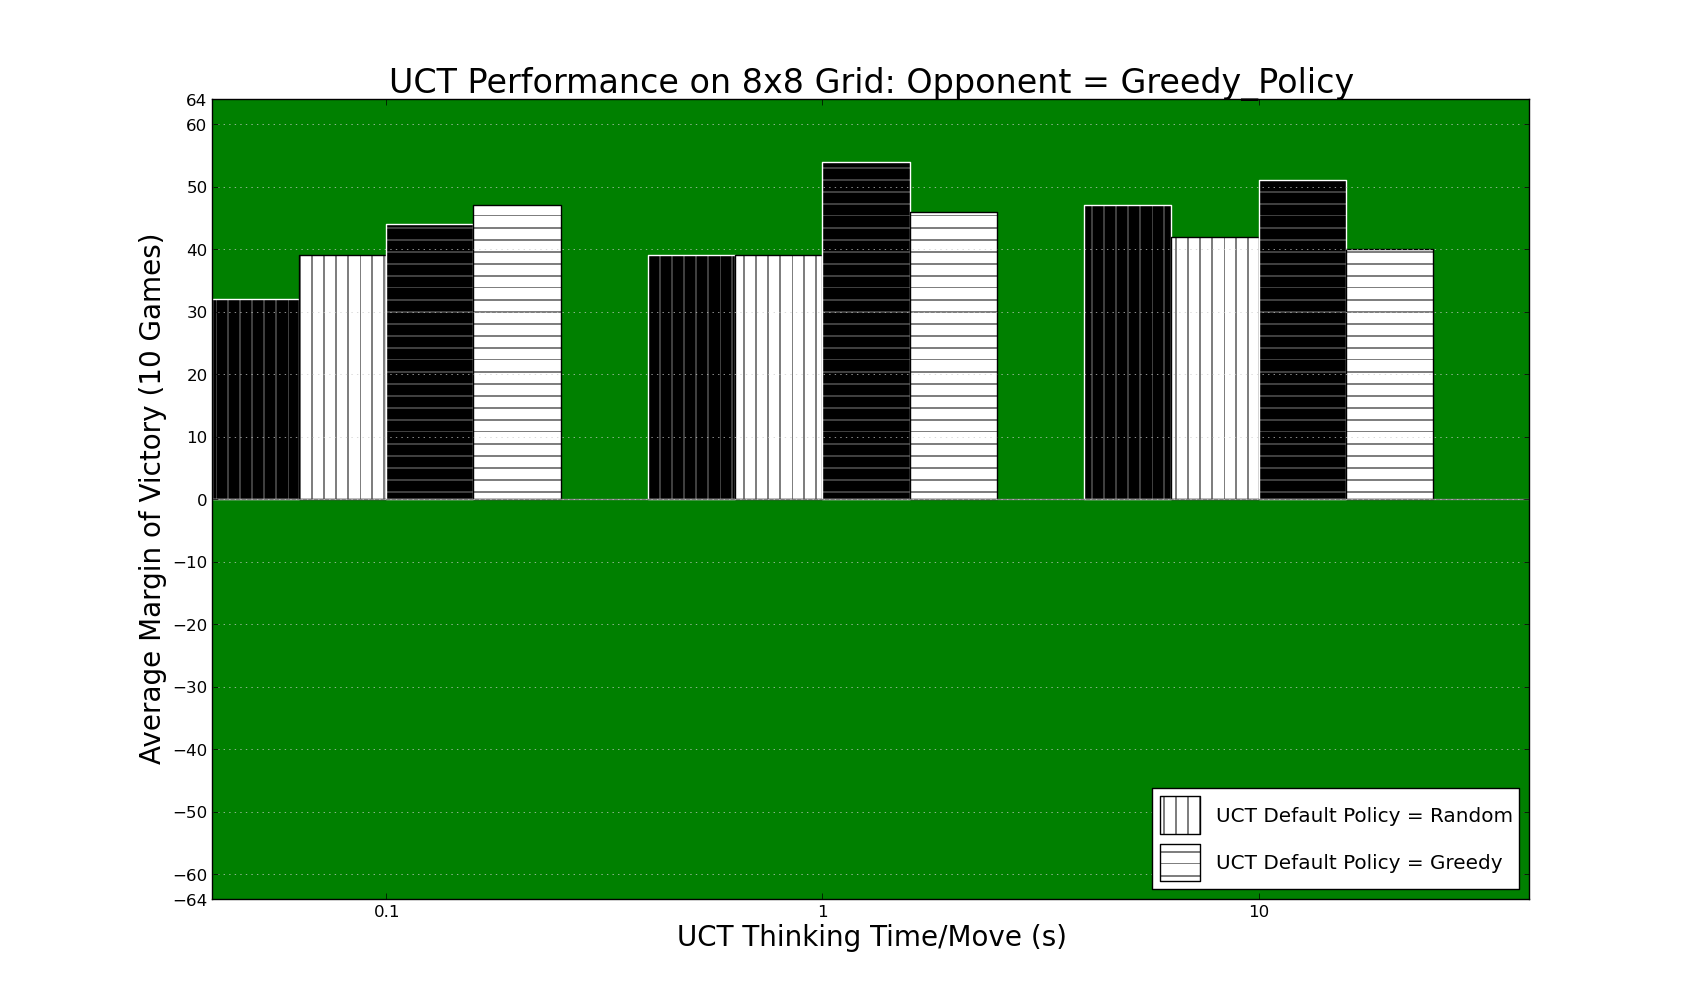
\includegraphics[scale=.4]{88_Greedy_Policy}
\end{center}
\end{figure}

\begin{figure}[!hp]
\begin{center}
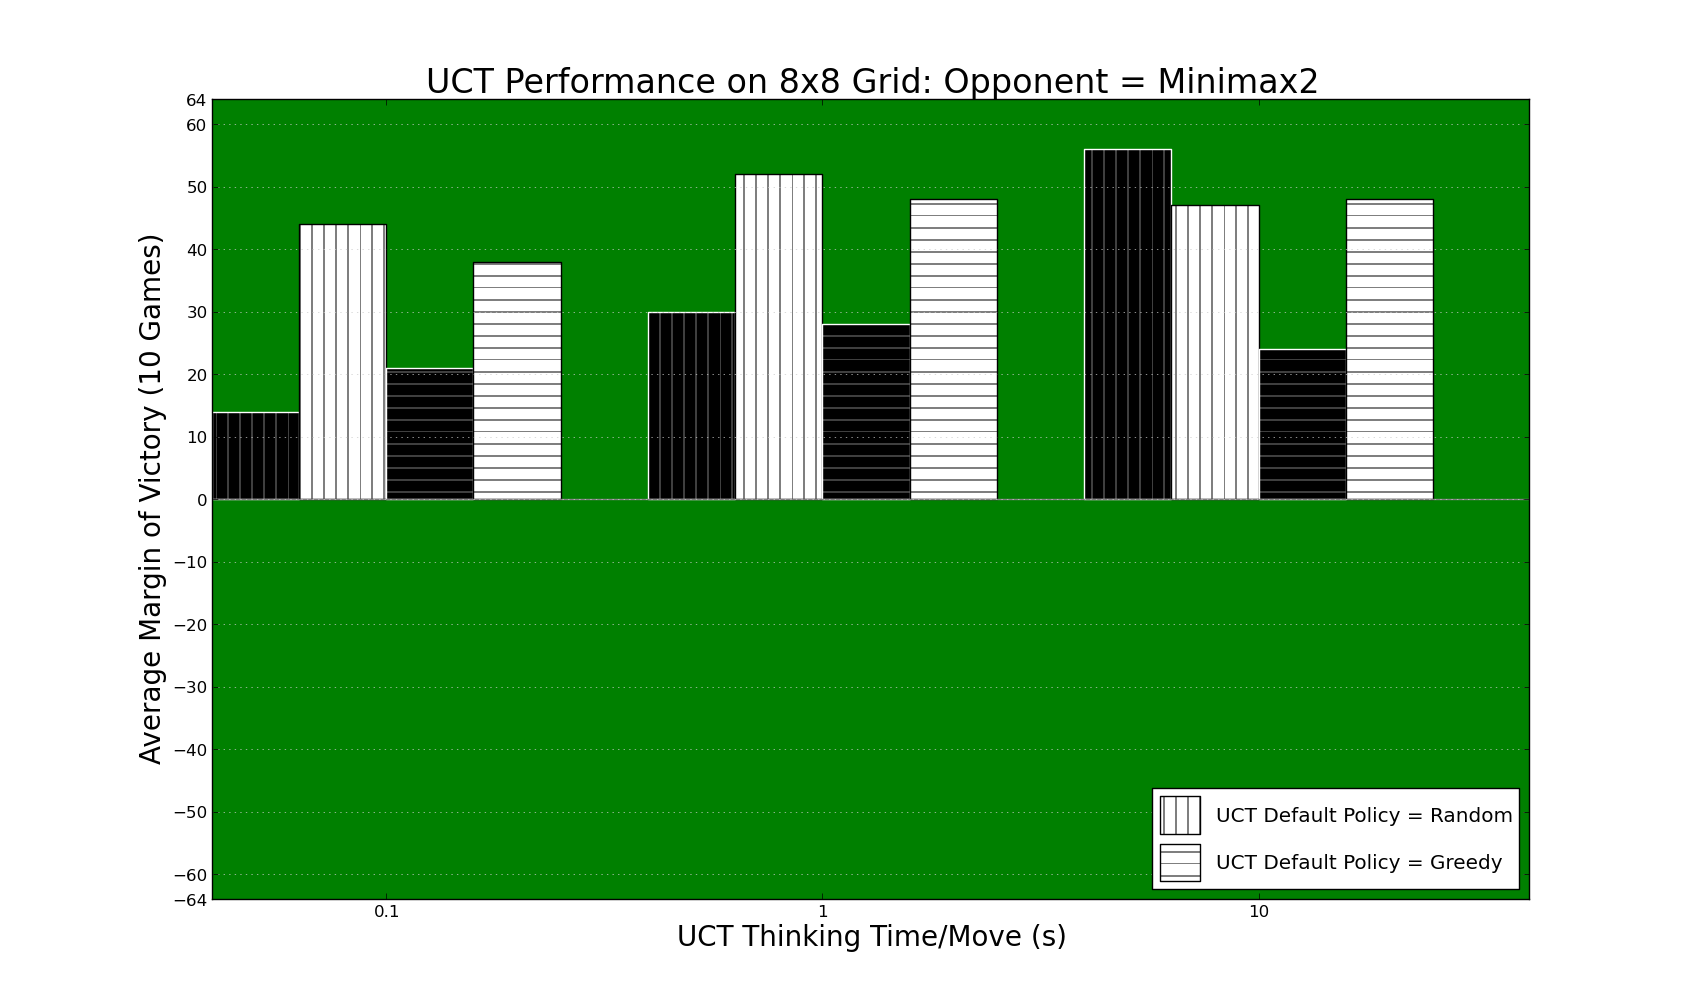
\includegraphics[scale=.4]{88_Minimax2}
\end{center}
\end{figure}

\begin{figure}[!hp]
\begin{center}
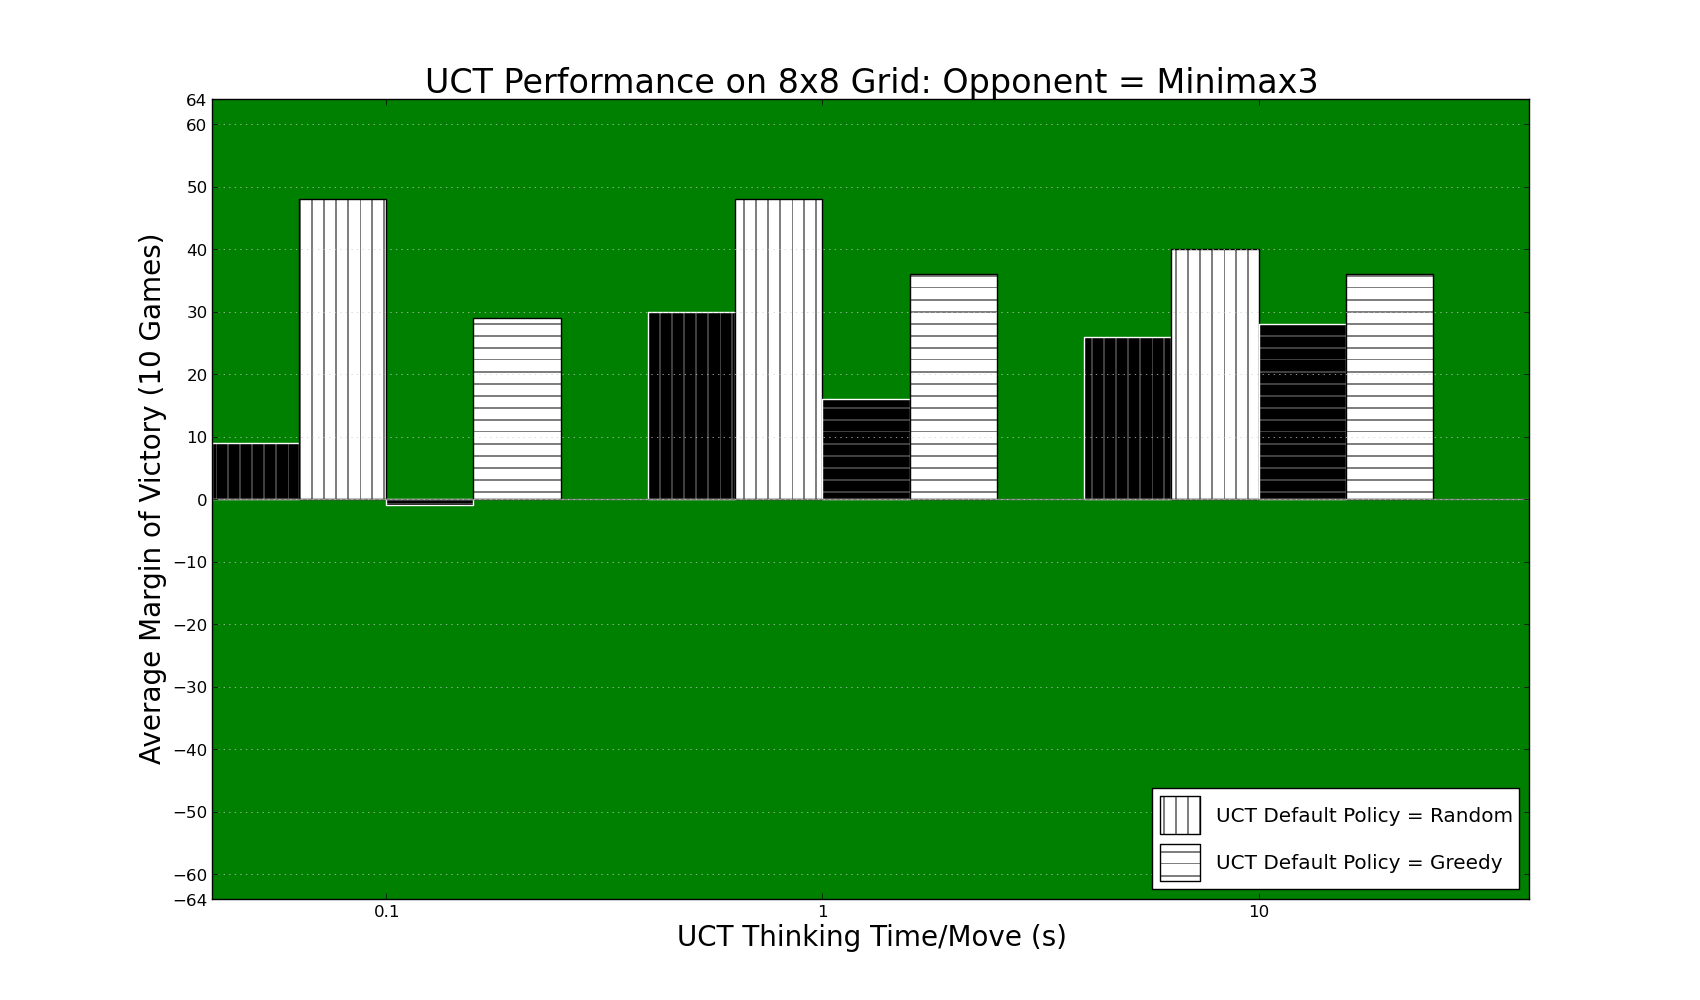
\includegraphics[scale=.4]{88_Minimax3}
\end{center}
\end{figure}

\begin{figure}[!h]
\begin{center}
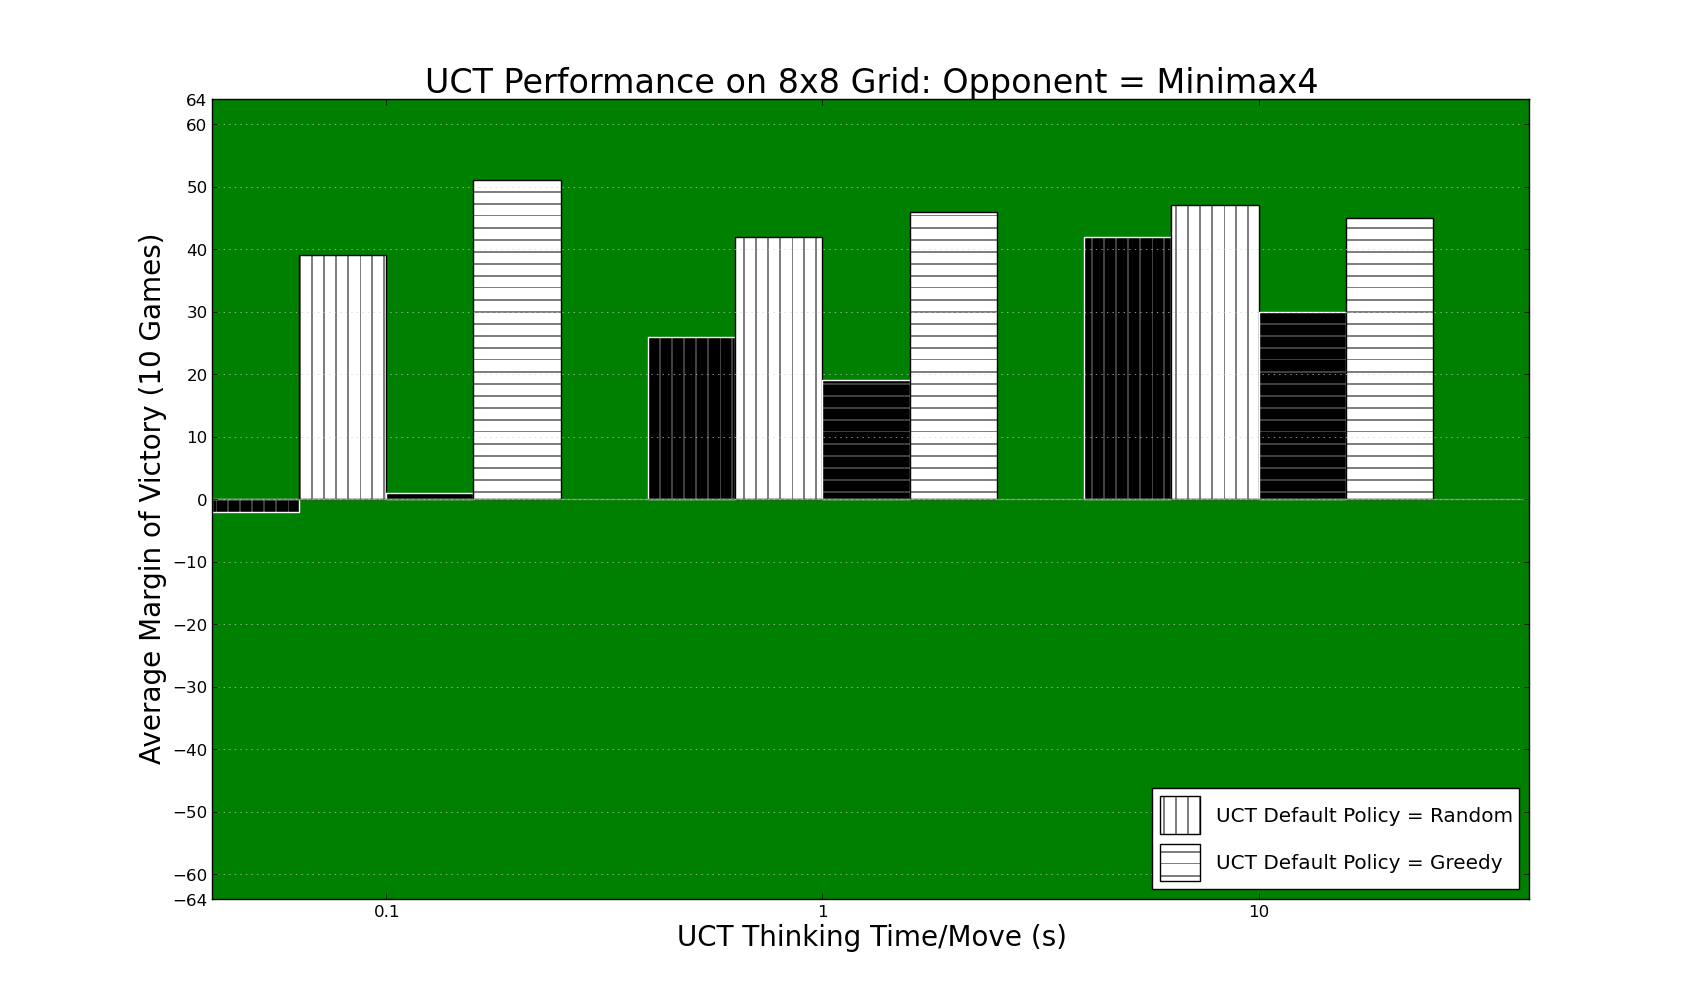
\includegraphics[scale=.4]{88_Minimax4}
\end{center}
\end{figure}

\pagebreak
\section{Discussion and Conclusion}
\label{conc}
Based on the above graphs, our UCT Othello playing agent performed quite well against multiple opponents. We were able to identify a few trends that confirm that our algorithm is working correctly.  First, the most obvious is that given a larger time budget, it is a general trend that the UCT algorithm performs better against all of the varied opponents. Second, against most opponents, it is the case that UCT wins on average by a larger margin when it is player 2 (white). After doing a bit of research on past Othello analysis it is largely agreed upon that the second player has an advantage in capturing more valuable positions on the board. Thus, in most Othello analyses, player 2 (white) has a higher probability of winning the game. 

This latter fact was especially amplified in playing more intelligent opponents (i.e. Minimax with 4 move lookahead) because when Minimax 4 went first, the moves that look better at the beginning of the game were selected, but given a higher probability of achieving more strategic places by moving second, the UCT algorithm typically made a comeback and won by a larger margin.

One surprise is that using the more ``intelligent" greedy policy as the default policy for simulation did not lead to more scucesful results in competition. It may be that the greater speed (meaning more simulated trajectories) and exploration resulting from the random policy offset the hopefully higher quality games resulting from the greedy policy.

Unfortunately due to the length of simulation time, we were not able to simulate and average over more than 10 games, and therefore there are a few outliers to the above trends.  However, we felt that the operation and performance of the UCT algorithm under various conditions was well-represented by the provided results.

\end{document}
